\documentclass[11pt,a4paper]{article}

% ── Packages ──────────────────────────────────────────────────────────
\usepackage[utf8]{inputenc}
\usepackage[T1]{fontenc}
\usepackage{lmodern}
\usepackage[margin=2.5cm]{geometry}
\usepackage{amsmath,amssymb,mathtools}
\usepackage{booktabs}
\usepackage{array}
\usepackage{longtable}
\usepackage{multirow}
\usepackage{enumitem}
\usepackage{fancyhdr}
\usepackage{titlesec}
\usepackage{float}
\usepackage{caption}
\usepackage{subcaption}
\usepackage{tikz}
\usepackage{pgfplots}
\usepackage{pifont}
\usepackage{xcolor}
\usepackage{hyperref}
\usepackage{tcolorbox}
\usepackage{listings}
\pgfplotsset{compat=1.18}
\usetikzlibrary{arrows.meta,positioning,calc,decorations.pathreplacing,
                 shapes.geometric,fit,backgrounds,matrix,chains}

\tcbuselibrary{skins,breakable,listings}

% ── Colors ────────────────────────────────────────────────────────────
\definecolor{appblue}{RGB}{40,100,180}
\definecolor{appgreen}{RGB}{40,140,60}
\definecolor{apporange}{RGB}{210,120,30}
\definecolor{appred}{RGB}{190,50,50}
\definecolor{apppurple}{RGB}{120,60,170}
\definecolor{codebg}{RGB}{248,248,252}
\definecolor{keybg}{RGB}{235,250,240}
\definecolor{archbg}{RGB}{245,245,255}
\definecolor{howbg}{RGB}{255,250,240}
\definecolor{dialectA}{RGB}{70,130,180}
\definecolor{dialectB}{RGB}{220,80,60}
\definecolor{dialectC}{RGB}{60,170,70}
\definecolor{dialectD}{RGB}{180,100,200}

% ── Environments ──────────────────────────────────────────────────────
\newtcolorbox{appbox}[1][]{
  colback=keybg, colframe=appgreen!80!black,
  fonttitle=\bfseries, title=#1,
  breakable, enhanced
}

\newtcolorbox{archbox}[1][]{
  colback=archbg, colframe=appblue!80!black,
  fonttitle=\bfseries, title={Architecture: #1},
  breakable, enhanced
}

\newtcolorbox{howbox}[1][]{
  colback=howbg, colframe=apporange!80!black,
  fonttitle=\bfseries, title={How It Works: #1},
  breakable, enhanced
}

\newtcolorbox{buildbox}[1][]{
  colback=codebg, colframe=gray!60!black,
  fonttitle=\bfseries, title={Building It: #1},
  breakable, enhanced
}

\lstdefinestyle{pythonstyle}{
  language=Python,
  basicstyle=\small\ttfamily,
  keywordstyle=\color{appblue}\bfseries,
  stringstyle=\color{appgreen},
  commentstyle=\color{gray}\itshape,
  backgroundcolor=\color{codebg},
  frame=single,
  framerule=0.4pt,
  rulecolor=\color{gray!40},
  breaklines=true,
  showstringspaces=false,
  tabsize=2,
  numbers=left,
  numberstyle=\tiny\color{gray},
  xleftmargin=2em,
}

\hypersetup{
    colorlinks=true,
    linkcolor=blue!70!black,
    citecolor=green!50!black,
    urlcolor=blue!60!black,
}

% ── Header ────────────────────────────────────────────────────────────
\pagestyle{fancy}
\fancyhf{}
\fancyhead[L]{\small\textit{Applications of EigenDialectos v3}}
\fancyhead[R]{\small\thepage}
\renewcommand{\headrulewidth}{0.4pt}

% ── Title ─────────────────────────────────────────────────────────────
\title{%
  \textbf{Applications of EigenDialectos v3}\\[0.3em]
  \Large What Can Be Built with Spectral Dialect Embeddings,\\
  How to Build It, and How It Works\\[0.5em]
  \large From Dialect Identification to Synthetic Dialect Generation
}
\author{EigenDialectos Project}
\date{April 2026}

\begin{document}
\maketitle
\thispagestyle{empty}

\begin{abstract}
EigenDialectos v3 produces a set of mathematical artifacts---word
embeddings, transformation matrices, eigendecompositions, and
spectral profiles---that encode the geometric structure of eight
Spanish dialect varieties. This document catalogs the applications
that these artifacts enable, ranging from real-time dialect
classification to synthetic dialect generation and computational
dialectometry. For each application, we explain the underlying
principle, the specific v3 artifacts it consumes, the system
architecture required to build it, and the concrete mechanisms by
which it operates. The applications span five domains:
\emph{identification and classification} (knowing which dialect),
\emph{transformation and transfer} (converting between dialects),
\emph{search and retrieval} (finding across dialects),
\emph{scientific tools} (measuring and mapping dialects), and
\emph{generative applications} (creating novel dialectal content).
\end{abstract}

\tableofcontents
\newpage

% ======================================================================
\section{Introduction: The Artifact Library}
\label{sec:artifacts}
% ======================================================================

Before describing applications, we must understand the artifacts that
v3 produces. Each application consumes one or more of these; knowing
which artifact does what is essential for understanding how each
application works.

\subsection{The Five Core Artifacts}

\begin{center}
\renewcommand{\arraystretch}{1.4}
\begin{tabular}{>{\bfseries}p{2.8cm} p{2.2cm} p{7.5cm}}
\toprule
\textbf{Artifact} & \textbf{Shape} & \textbf{What it encodes} \\
\midrule
Word embeddings $E_v$ &
  $(V \times 384)$ \newline per variety &
  A 384-dimensional vector for each of the $V \approx 10{,}800$ words in
  each dialect variety $v$. After Procrustes alignment, shared words
  occupy similar positions; dialectal words diverge. \\

Transformation matrix $W_{v}$ &
  $(384 \times 384)$ \newline per variety &
  The linear map from the reference dialect (ES\_PEN) to variety $v$:
  $E_v \approx E_{\text{PEN}} \cdot W_v$. Encodes how variety $v$
  deforms the reference space. \\

Eigendecomposition $P_v, \boldsymbol{\lambda}_v$ &
  $P_v$: $(384 \times 384)$ \newline $\boldsymbol{\lambda}_v$: $(384,)$ &
  $W_v = P_v \,\text{diag}(\boldsymbol{\lambda}_v)\, P_v^{-1}$.
  The eigenvectors $P_v$ are the \emph{axes of dialectal variation};
  the eigenvalues $\boldsymbol{\lambda}_v$ are the \emph{magnitudes}
  along each axis. Together they form a dialect's
  \emph{spectral fingerprint}. \\

Vocabulary &
  $(V,)$ list &
  The shared word list, ordered consistently across all embedding
  matrices. Each word has a per-dialect vector, enabling direct
  comparison. \\

Trained model &
  BETO+LoRA \newline + projection &
  The fine-tuned Transformer (110M frozen + 2.7M LoRA) and
  projection head ($768 \to 384$). Can embed arbitrary new text
  into the dialect geometry. \\
\bottomrule
\end{tabular}
\end{center}

\subsection{Dependency Map}

\begin{center}
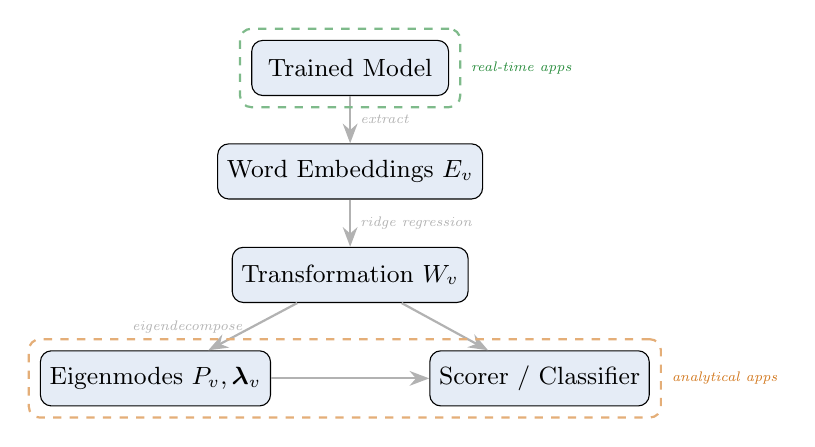
\begin{tikzpicture}[
  art/.style={draw, rounded corners=4pt, minimum height=0.7cm,
              minimum width=2.5cm, font=\small, align=center},
  arr/.style={-{Stealth[length=2.5mm]}, thick, gray!60},
  node distance=0.6cm and 1.5cm
]
\node[art, fill=appblue!12] (model) {Trained Model};
\node[art, fill=appblue!12, below=of model] (emb) {Word Embeddings $E_v$};
\node[art, fill=appblue!12, below=of emb] (W) {Transformation $W_v$};
\node[art, fill=appblue!12, below left=0.6cm and -0.5cm of W] (eigen) {Eigenmodes $P_v, \boldsymbol{\lambda}_v$};
\node[art, fill=appblue!12, below right=0.6cm and -0.5cm of W] (scorer) {Scorer / Classifier};

\draw[arr] (model) -- (emb) node[midway, right, font=\tiny\itshape] {extract};
\draw[arr] (emb) -- (W) node[midway, right, font=\tiny\itshape] {ridge regression};
\draw[arr] (W) -- (eigen) node[midway, left, font=\tiny\itshape] {eigendecompose};
\draw[arr] (W) -- (scorer);
\draw[arr] (eigen) -- (scorer);

% Application clusters
\node[draw, dashed, rounded corners, appgreen!60, thick,
      fit=(model), inner sep=4pt, label={[font=\tiny\itshape, appgreen]right:real-time apps}] {};
\node[draw, dashed, rounded corners, apporange!60, thick,
      fit=(eigen)(scorer), inner sep=4pt, label={[font=\tiny\itshape, apporange]right:analytical apps}] {};
\end{tikzpicture}
\end{center}

Applications that need to process \emph{new, unseen text} (dialect
identification, chatbots, monitoring) require the trained model.
Applications that operate on \emph{the vocabulary} (dialectometry,
dialect algebra, mapping) only need the embeddings and their
decompositions.

% ======================================================================
\part{Identification and Classification}
% ======================================================================

% ----------------------------------------------------------------------
\section{Application 1: Real-Time Dialect Identification API}
\label{sec:app-identify}
% ----------------------------------------------------------------------

\begin{appbox}[What it does]
Given any Spanish text---a tweet, a customer support message, a
paragraph from a novel---the system returns a probability distribution
over the eight dialect varieties, plus a confidence score and the
top-3 most diagnostic words.
\end{appbox}

\subsection{Why it is useful}

\begin{itemize}[nosep]
  \item \textbf{Content routing:} a multinational customer support
        center automatically routes tickets to agents who speak the
        caller's variety.
  \item \textbf{Market research:} a brand monitors social media and
        segments commentary by dialect, revealing regional sentiment
        differences.
  \item \textbf{Corpus curation:} researchers building dialect-specific
        datasets can automatically label large text collections.
\end{itemize}

\subsection{Which artifacts it uses}

\begin{center}
\begin{tabular}{ll}
\toprule
\textbf{Artifact} & \textbf{Role} \\
\midrule
Trained model & Embeds input text into the 384-d dialect space \\
Eigendecompositions $P_v, \boldsymbol{\lambda}_v$ &
  Reference spectral profiles for each dialect \\
Word embeddings $E_v$ & Per-word dialect affinities for
  interpretability \\
Vocabulary & Word lookup for scoring \\
\bottomrule
\end{tabular}
\end{center}

\begin{howbox}{Dialect identification}
\begin{enumerate}[nosep]
  \item \textbf{Tokenize and embed.} The input text is tokenized by
    BETO's tokenizer and passed through the fine-tuned Transformer +
    projection head, producing one 384-d unit-norm vector per token.

  \item \textbf{Aggregate to a text centroid.} Token vectors are
    averaged (optionally IDF-weighted, where IDF is computed from
    spectral variance---words that vary more across dialects get
    higher weight) into a single 384-d centroid $\mathbf{c}$.

  \item \textbf{Project onto eigenmodes.} For each dialect $v$, the
    centroid is projected onto the eigenaxes:
    $\mathbf{a}_v = P_v^{-1} \mathbf{c}$. The resulting
    \emph{activation vector} $\mathbf{a}_v$ measures how strongly
    the text activates each dialectal axis.

  \item \textbf{Compare to reference profiles.} During setup, the
    system pre-computes a reference activation profile
    $\bar{\mathbf{a}}_v$ for each dialect (the mean activation
    over that dialect's corpus). The distance
    $d_v = \|\mathbf{a}_v - \bar{\mathbf{a}}_v\|$ measures how
    far the input is from each dialect's ``center of gravity'' in
    spectral space.

  \item \textbf{Score.} Distances are converted to probabilities
    via softmax: $p_v \propto \exp(-d_v / T)$. Per-word affinities
    are aggregated via naive Bayes for an additional signal, and the
    two scores are combined.

  \item \textbf{Interpret.} For each word in the input, the system
    looks up its per-dialect affinity (divergence from the
    cross-variety mean). The top-$k$ most discriminative words are
    returned alongside the probability distribution.
\end{enumerate}
\end{howbox}

\begin{archbox}{REST API}
\begin{center}
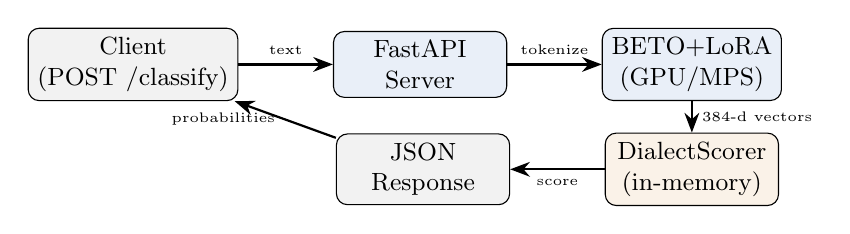
\begin{tikzpicture}[
  comp/.style={draw, rounded corners=4pt, minimum height=0.8cm,
               minimum width=2.2cm, font=\small, align=center},
  arr/.style={-{Stealth[length=2.5mm]}, thick},
  node distance=0.4cm and 1.2cm
]
\node[comp, fill=gray!10] (client) {Client\\(POST /classify)};
\node[comp, fill=appblue!10, right=of client] (api) {FastAPI\\Server};
\node[comp, fill=appblue!10, right=of api] (model) {BETO+LoRA\\(GPU/MPS)};
\node[comp, fill=apporange!10, below=of model] (scorer) {DialectScorer\\(in-memory)};
\node[comp, fill=gray!10, left=of scorer] (resp) {JSON\\Response};

\draw[arr] (client) -- (api) node[midway, above, font=\tiny] {text};
\draw[arr] (api) -- (model) node[midway, above, font=\tiny] {tokenize};
\draw[arr] (model) -- (scorer) node[midway, right, font=\tiny] {384-d vectors};
\draw[arr] (scorer) -- (resp) node[midway, below, font=\tiny] {score};
\draw[arr] (resp) -- (client) node[midway, left, font=\tiny] {probabilities};
\end{tikzpicture}
\end{center}

The trained model and scorer are loaded once at startup. The model
lives on GPU/MPS; the eigendecompositions and embeddings live in CPU
RAM ($\sim$300~MB for 8 varieties $\times$ 10,800 words $\times$
384 dims). Inference latency: $\sim$20--50\,ms per request for texts
up to 256 tokens.
\end{archbox}

\begin{buildbox}{Key components}
\begin{enumerate}[nosep]
  \item Load the fine-tuned BETO+LoRA checkpoint and projection head.
  \item Load the pre-computed eigendecompositions and word embeddings.
  \item Instantiate a \texttt{DialectScorer} with the embeddings,
        vocabulary, and decompositions.
  \item Wrap in a FastAPI endpoint that accepts text and returns a
        JSON object with per-dialect probabilities, confidence, and
        top diagnostic words.
  \item For batch processing (corpus labeling), add a
        \texttt{/batch\_classify} endpoint that processes lists of
        texts with internal batching for GPU efficiency.
\end{enumerate}
\end{buildbox}

% ----------------------------------------------------------------------
\section{Application 2: Dialect-Aware Spam and Content Filtering}
\label{sec:app-filter}
% ----------------------------------------------------------------------

\begin{appbox}[What it does]
A content moderation system that understands dialectal variation.
Instead of flagging Caribbean or Rioplatense slang as ``unknown'' or
``potentially offensive,'' it recognizes the dialect and applies
dialect-appropriate moderation rules.
\end{appbox}

\subsection{The problem it solves}

Standard NLP moderation tools are typically trained on a single
prestige variety of Spanish (usually Peninsular or Mexican). Words
like \emph{coger} (``to take/catch'' in most of Latin America,
vulgar in Rioplatense/Mexican), \emph{bicho} (``bug'' in most
dialects, slang in Caribbean), or \emph{joder} (mild in Peninsular,
strong in Latin American) trigger false positives or false negatives
because the tools are dialect-blind.

\begin{howbox}{Dialect-conditional moderation}
\begin{enumerate}[nosep]
  \item \textbf{Classify the dialect} using Application~1.
  \item \textbf{Select the appropriate lexicon.} Each dialect has a
    curated moderation lexicon where polysemous words are annotated
    with their dialect-specific valence.
  \item \textbf{Run moderation with dialect context.} The word
    embeddings from v3 provide per-dialect vector representations;
    words that are semantically neutral in dialect $v$ will cluster
    with neutral words in $E_v$, even if they cluster with offensive
    words in $E_{v'}$.
  \item \textbf{Adjust confidence.} If the dialect classifier is
    uncertain (e.g., 40\% Caribbean, 35\% Mexican), the system
    flags for human review rather than auto-moderating.
\end{enumerate}
\end{howbox}

The key insight is that the per-dialect word embeddings $E_v$ encode
\emph{dialect-specific semantics}: the same surface form maps to
different vectors in different dialect spaces, reflecting its actual
usage and connotation within that community.

% ======================================================================
\part{Transformation and Transfer}
% ======================================================================

% ----------------------------------------------------------------------
\section{Application 3: Cross-Dialectal Style Transfer}
\label{sec:app-transfer}
% ----------------------------------------------------------------------

\begin{appbox}[What it does]
Given a text written in one Spanish dialect, the system produces a
version in another dialect, preserving meaning while shifting
vocabulary, idiom, and register to match the target variety.

\medskip
\emph{Input (Rioplatense):} ``Che, vos ten\'es que tomar el colectivo
en la esquina.''

\emph{Output (Peninsular):} ``Oye, t\'u tienes que coger el
autob\'us en la esquina.''

\emph{Output (Mexican):} ``Oye, t\'u tienes que tomar el cami\'on en
la esquina.''
\end{appbox}

\subsection{Why this is hard without eigenv3}

Dialect transfer is not machine translation. The source and target
share 95\%+ of their grammar and vocabulary. The differences are
sparse but socially critical: a wrong pronoun (\emph{vos} vs.\
\emph{t\'u}), a wrong lexical choice (\emph{colectivo} vs.\
\emph{autob\'us} vs.\ \emph{cami\'on}), or a wrong phonological
spelling (\emph{pa'} vs.\ \emph{para}) immediately breaks the
illusion. A generic translation model has no mechanism to make these
precise, sparse substitutions.

\subsection{Which artifacts it uses}

\begin{center}
\begin{tabular}{ll}
\toprule
\textbf{Artifact} & \textbf{Role} \\
\midrule
Transformation matrices $W_v$ & Map source $\to$ target dialect space \\
Word embeddings $E_v$ & Source and target word vectors for
  nearest-neighbor lookup \\
Eigendecompositions & Identify which words sit on dialectal axes
  (candidates for substitution) \\
Vocabulary & Candidate substitution pool \\
\bottomrule
\end{tabular}
\end{center}

\begin{howbox}{Dialect transfer via eigenmode routing}
\begin{enumerate}
  \item \textbf{Identify dialectal words.} For each word in the input,
    compute its \emph{dialectal salience}: the magnitude of its
    projection onto the top eigenmodes of $W_{\text{source}}$. Words
    with high salience are dialect-specific; words with low salience
    are shared pan-Hispanic vocabulary and should not be changed.

    Formally, given word $w$ with embedding $\mathbf{e}_w$ in the
    source dialect:
    \[
    \text{salience}(w) = \sum_{k=1}^{K}
    |\lambda_k| \cdot |(P^{-1}_{\text{source}} \cdot \mathbf{e}_w)_k|
    \]
    where $K$ is the number of top eigenmodes considered (typically
    10--20).

  \item \textbf{Transform to target space.} Apply the transformation
    chain:
    \[
    \mathbf{e}'_w = \mathbf{e}_w \cdot W_{\text{source}}^{-1}
                                  \cdot W_{\text{target}}
    \]
    This maps the word from the source dialect's coordinate system
    through the reference (ES\_PEN) and into the target dialect's
    space.

  \item \textbf{Find the nearest target word.} For each transformed
    vector $\mathbf{e}'_w$, find the nearest neighbor in the target
    embedding matrix $E_{\text{target}}$:
    \[
    w' = \arg\max_{u \in \text{vocab}}
    \frac{\mathbf{e}'_w \cdot E_{\text{target}}[u]}
         {\|\mathbf{e}'_w\| \cdot \|E_{\text{target}}[u]\|}
    \]
    If $w' = w$ (the nearest neighbor is the same word), no
    substitution is needed---the word is shared.

  \item \textbf{Apply substitutions.} Replace dialect-specific words
    (high salience + changed nearest neighbor) with their target
    equivalents. Leave shared words untouched.

  \item \textbf{Post-process.} Apply morphological agreement rules
    (gender, number, verb conjugation) to ensure grammaticality.
    A rule-based layer handles the pronoun system (\emph{vos}
    $\leftrightarrow$ \emph{t\'u} $\leftrightarrow$ \emph{usted})
    and associated verb forms.
\end{enumerate}
\end{howbox}

\begin{archbox}{Transfer pipeline}
\begin{center}
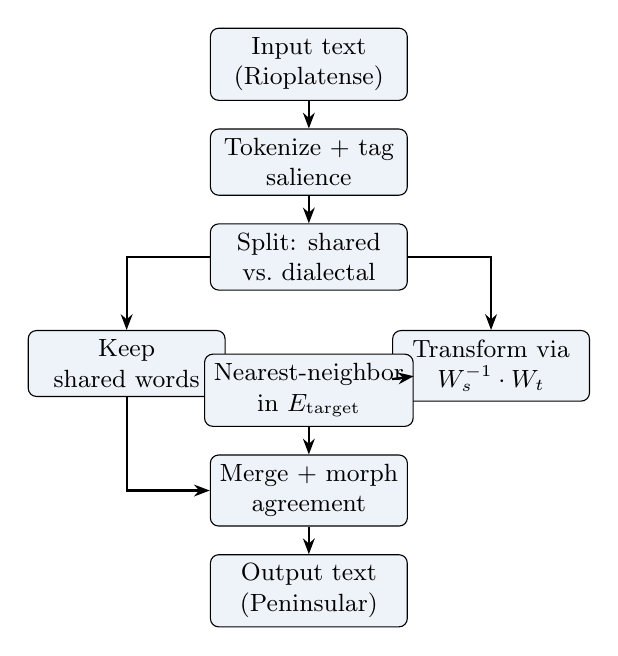
\begin{tikzpicture}[
  pipestep/.style={draw, rounded corners=3pt, minimum height=0.65cm,
               minimum width=2.5cm, font=\small, align=center,
               fill=appblue!8},
  arr/.style={-{Stealth[length=2mm]}, thick},
  node distance=0.35cm
]
\node[pipestep] (input) {Input text\\(Rioplatense)};
\node[pipestep, below=of input] (tokenize) {Tokenize + tag\\salience};
\node[pipestep, below=of tokenize] (classify) {Split: shared\\vs.\ dialectal};
\node[pipestep, below left=0.5cm and -0.2cm of classify] (keep) {Keep\\shared words};
\node[pipestep, below right=0.5cm and -0.2cm of classify] (transform) {Transform via\\$W^{-1}_s \cdot W_t$};
\node[pipestep, below=0.8cm of classify] (nn) {Nearest-neighbor\\in $E_{\text{target}}$};
\node[pipestep, below=of nn] (merge) {Merge + morph\\agreement};
\node[pipestep, below=of merge] (output) {Output text\\(Peninsular)};

\draw[arr] (input) -- (tokenize);
\draw[arr] (tokenize) -- (classify);
\draw[arr] (classify) -| (keep);
\draw[arr] (classify) -| (transform);
\draw[arr] (keep) |- (merge);
\draw[arr] (transform) -- (nn);
\draw[arr] (nn) -- (merge);
\draw[arr] (merge) -- (output);
\end{tikzpicture}
\end{center}
\end{archbox}

\subsection{Limitations and hybrid approach}

Pure eigenmode-based transfer handles lexical substitutions well but
struggles with syntactic dialect differences (e.g., Rioplatense
\emph{vos ten\'es} $\to$ Peninsular \emph{t\'u tienes} requires
understanding verb morphology, not just word vectors). A production
system would combine:
\begin{itemize}[nosep]
  \item Eigenmode-based lexical transfer (v3 artifacts).
  \item Rule-based morphological transformation (pronoun/verb tables).
  \item Optionally, an LLM post-editing pass for fluency.
\end{itemize}

% ----------------------------------------------------------------------
\section{Application 4: Content Localization Engine}
\label{sec:app-localization}
% ----------------------------------------------------------------------

\begin{appbox}[What it does]
A platform that takes marketing copy, UI strings, or editorial
content written in one Spanish variety and produces localized
versions for all eight markets simultaneously, highlighting which
words were changed and why.
\end{appbox}

\subsection{How it differs from Application 3}

Style transfer (Application~3) operates on arbitrary text and aims for
natural output. Localization operates on \emph{controlled content}
(product descriptions, app UI, help articles) and aims for
\emph{brand-consistent, accurate} output with full audit trails.

\begin{howbox}{Localization pipeline}
\begin{enumerate}[nosep]
  \item \textbf{Scan for dialectally sensitive terms.} Using per-word
    dialect affinities from $E_v$, flag every word that has
    significantly different embeddings across target markets. A word
    is flagged if:
    \[
    \max_{v, v'} \|E_v[w] - E_{v'}[w]\| > \theta
    \]
    for a threshold $\theta$ calibrated against known regionalisms.

  \item \textbf{Propose substitutions per market.} For each flagged
    word, use the transformation $W_s^{-1} W_t$ to find the target
    equivalent and present it to a human reviewer with:
    \begin{itemize}[nosep]
      \item The source word and its dialect affinity profile.
      \item The proposed target word and cosine similarity.
      \item The eigenmode(s) driving the difference (e.g., ``mode 3:
            transportation vocabulary'').
    \end{itemize}

  \item \textbf{Build a translation memory.} Approved substitutions
    are cached. Over time, the system builds a per-brand, per-market
    translation memory that accelerates future localizations.

  \item \textbf{Generate all eight versions.} Apply the approved
    substitution map to produce all market variants from a single
    source text.
\end{enumerate}
\end{howbox}

\subsection{The eigenmode advantage}

Without eigenmodes, localization relies on curated synonym dictionaries
(expensive, incomplete, rapidly outdated). Eigenmodes provide:
\begin{itemize}[nosep]
  \item \textbf{Automatic discovery:} the system finds dialectal
    terms the dictionary missed, because the eigenmodes encode
    \emph{all} axes of variation, not just known lexical pairs.
  \item \textbf{Interpretability:} each substitution can be traced
    to a specific eigenmode (``transportation,'' ``food,''
    ``forms of address''), making review meaningful.
  \item \textbf{Completeness:} the eigenvalue spectrum tells you how
    many axes of variation exist between any two markets, providing a
    quantitative measure of localization effort.
\end{itemize}

% ======================================================================
\part{Search and Retrieval}
% ======================================================================

% ----------------------------------------------------------------------
\section{Application 5: Cross-Dialectal Semantic Search}
\label{sec:app-search}
% ----------------------------------------------------------------------

\begin{appbox}[What it does]
A search engine where a user querying \emph{``pileta''} (Rioplatense
for swimming pool) also retrieves documents containing
\emph{``piscina''} (Peninsular/Mexican), \emph{``alberca''}
(Mexican), and \emph{``piscinita''} (Caribbean diminutive)---even
though these are different surface forms---because the system
understands they occupy the same position in their respective
dialect spaces.
\end{appbox}

\begin{howbox}{Cross-dialectal retrieval}
\begin{enumerate}[nosep]
  \item \textbf{Index documents.} Each document is embedded into the
    384-d projection space by the trained model. Additionally, for
    each content word, its \emph{reference-space} embedding is stored:
    $\mathbf{e}_{\text{ref}}(w) = E_v[w] \cdot W_v^{-1}$. This maps
    every dialect's words into the common reference space (ES\_PEN).

  \item \textbf{Process queries.} The query is classified
    (Application~1) and its content words are similarly mapped to
    reference space.

  \item \textbf{Match in reference space.} Because all words from all
    dialects have been projected into the same reference frame,
    ``pileta'' (mapped from Rioplatense) and ``piscina'' (mapped
    from Peninsular) land at nearby positions.

  \item \textbf{Rank.} Standard semantic similarity (cosine of
    document centroid vs.\ query centroid in reference space), with a
    boost for documents whose source dialect matches the query dialect
    (if desired).
\end{enumerate}
\end{howbox}

\begin{archbox}{Search system}
\begin{center}
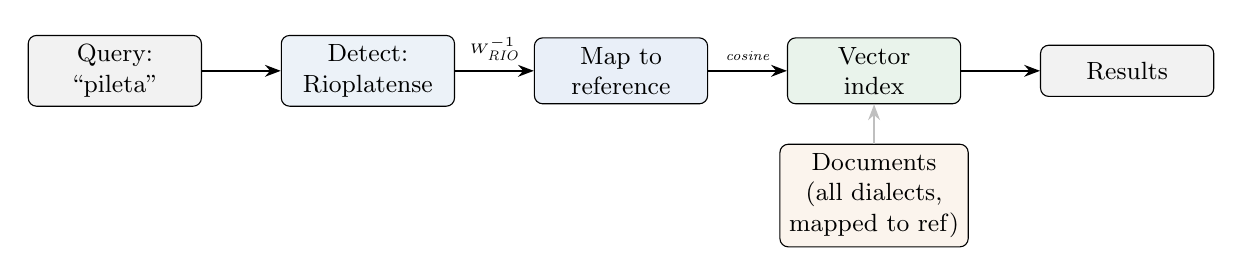
\begin{tikzpicture}[
  comp/.style={draw, rounded corners=3pt, minimum height=0.65cm,
               minimum width=2.2cm, font=\small, align=center},
  arr/.style={-{Stealth[length=2mm]}, thick},
  node distance=0.35cm and 1cm
]
\node[comp, fill=gray!10] (query) {Query:\\``pileta''};
\node[comp, fill=dialectA!10, right=of query] (detect) {Detect:\\Rioplatense};
\node[comp, fill=appblue!10, right=of detect] (ref) {Map to\\reference};
\node[comp, fill=appgreen!10, right=of ref] (index) {Vector\\index};
\node[comp, fill=gray!10, right=of index] (results) {Results};

\draw[arr] (query) -- (detect);
\draw[arr] (detect) -- (ref)
  node[midway, above, font=\tiny\itshape] {$W_{\text{RIO}}^{-1}$};
\draw[arr] (ref) -- (index)
  node[midway, above, font=\tiny\itshape] {cosine};
\draw[arr] (index) -- (results);

\node[comp, fill=apporange!8, below=0.5cm of index] (docs)
  {Documents\\(all dialects,\\mapped to ref)};
\draw[arr, gray!50] (docs) -- (index);
\end{tikzpicture}
\end{center}
\end{archbox}

The critical enabler is Procrustes alignment: because all eight
dialect spaces are aligned to a common reference via shared anchor
words, the transformation $W_v^{-1}$ reliably maps dialect-specific
terms into a shared coordinate system where synonyms across dialects
become neighbors.

% ----------------------------------------------------------------------
\section{Application 6: Dialect-Aware Recommendation}
\label{sec:app-recommend}
% ----------------------------------------------------------------------

\begin{appbox}[What it does]
A content platform (news, entertainment, e-commerce) that detects the
user's dialect from their search queries and interaction text, then
prioritizes content written in or localized for that variety.
\end{appbox}

\begin{howbox}{Recommendation signal}
\begin{enumerate}[nosep]
  \item \textbf{Build a user dialect profile.} Accumulate dialect
    classification results (Application~1) over the user's recent
    interactions. The profile is a running average of the 8-way
    probability distribution.

  \item \textbf{Compute content dialect affinity.} Each content item
    is pre-classified. Its dialect probability vector becomes a
    metadata tag.

  \item \textbf{Boost matching content.} The recommendation score for
    content $c$ given user $u$ is augmented by the cosine similarity
    between their dialect probability vectors:
    \[
    \text{score}(u, c) = \text{relevance}(u, c) +
    \alpha \cdot \mathbf{d}_u \cdot \mathbf{d}_c
    \]
    where $\alpha$ controls the dialect-matching weight.
\end{enumerate}
\end{howbox}

This requires only Application~1 applied to both user text and content
text. No transformation matrices or eigenmodes needed---just the
classifier.

% ======================================================================
\part{Scientific and Research Tools}
% ======================================================================

% ----------------------------------------------------------------------
\section{Application 7: Computational Dialectometry}
\label{sec:app-dialectometry}
% ----------------------------------------------------------------------

\begin{appbox}[What it does]
A quantitative dialectology platform that computes continuous
distances between dialect varieties, identifies axes of variation,
maps isoglosses, and produces publication-quality visualizations---all
from the spectral structure of the embedding matrices.
\end{appbox}

\subsection{Spectral distance}

The eigenvalue spectrum $\boldsymbol{\lambda}_v$ is a compact
fingerprint of how variety $v$ deforms the reference space. The
distance between two varieties can be measured as:
\[
d_{\text{spectral}}(v, v')
= \left\|\,|\boldsymbol{\lambda}_v| - |\boldsymbol{\lambda}_{v'}|\,\right\|_2
\]
This is a single number that quantifies how differently two dialects
transform Spanish.

\begin{howbox}{Dialectometric analysis}
\begin{enumerate}[nosep]
  \item \textbf{Distance matrix.} Compute $d_{\text{spectral}}$ for
    all $\binom{8}{2} = 28$ dialect pairs.

  \item \textbf{Hierarchical clustering.} Apply agglomerative
    clustering to the distance matrix to produce a dialect dendrogram.
    The expected structure: Peninsular clusters with Canarian;
    Rioplatense is an outlier; Mexican, Caribbean, Chilean form a
    cluster; Andean forms bridge to Andean-Bolivian.

  \item \textbf{Eigenmode interpretation.} For each eigenmode $k$ of
    each variety, the analyzer identifies the top-$n$ words with the
    highest loading magnitude. This reveals \emph{what} each axis of
    variation is about (e.g., mode 1: pronouns and forms of address;
    mode 3: transportation lexicon; mode 7: food vocabulary).

  \item \textbf{Shared vs.\ unique axes.} The analyzer compares
    eigenvectors across dialects (via cosine similarity of
    corresponding eigenmode loadings). Modes shared across many
    dialects represent pan-Hispanic variation; modes unique to one
    dialect represent that variety's distinctive features.

  \item \textbf{Effective rank.} The effective rank
    (exponential of Shannon entropy of normalized eigenvalue
    magnitudes) measures how many independent axes of variation a
    dialect has. A high effective rank means the dialect differs
    from the reference along many dimensions; a low rank means the
    differences are concentrated in a few.
\end{enumerate}
\end{howbox}

\subsection{Isogloss mapping}

An \textbf{isogloss} is a geographic boundary separating regions that
differ in a specific linguistic feature. Traditionally, isoglosses
are drawn by hand from fieldwork data. Eigenmodes automate this:

\begin{enumerate}[nosep]
  \item Pick an eigenmode $k$ (e.g., the transportation lexicon mode).
  \item For each variety, extract the eigenvalue $\lambda_{v,k}$.
  \item Varieties where $|\lambda_{v,k}|$ is large participate in
    this axis of variation; varieties where it is near 1.0 do not.
  \item The boundary between participating and non-participating
    varieties is a computationally derived isogloss.
\end{enumerate}

% ----------------------------------------------------------------------
\section{Application 8: Dialect Algebra and Synthetic Dialects}
\label{sec:app-algebra}
% ----------------------------------------------------------------------

\begin{appbox}[What it does]
The eigendecomposition enables arithmetic on dialects: interpolating
between two varieties, computing dialect analogies (``A is to B as C
is to ?''), and even constructing hypothetical dialects that have
never existed.
\end{appbox}

\subsection{Spectral interpolation}

Given two dialects $v_1$ and $v_2$ with eigenvalue spectra
$\boldsymbol{\lambda}_1$ and $\boldsymbol{\lambda}_2$, we can create
a continuous path between them:
\[
\boldsymbol{\lambda}_\alpha
= (1 - \alpha)\,\boldsymbol{\lambda}_1
+ \alpha\,\boldsymbol{\lambda}_2, \qquad \alpha \in [0, 1]
\]
At $\alpha = 0$ we have dialect 1; at $\alpha = 1$, dialect 2; at
$\alpha = 0.5$, a hypothetical ``midpoint'' dialect.

\begin{howbox}{What interpolation reveals}
Walking the interpolation path and monitoring which words change
reveals the \emph{order of dialectal features}: the features that
change first (at small $\alpha$) are the most salient differences
between the two dialects; features that change last are the most
deeply shared.

Example: interpolating from Rioplatense to Mexican, the pronoun
system (\emph{vos} $\to$ \emph{t\'u}) changes at $\alpha \approx
0.15$, while basic vocabulary (\emph{casa}, \emph{agua}) remains
stable until $\alpha > 0.9$. This quantifies the intuition that
pronoun use is more dialectally marked than basic nouns.
\end{howbox}

\subsection{Dialect analogies}

The algebra module solves analogies of the form ``Rioplatense is to
Peninsular as Caribbean is to ?'' by:
\[
\boldsymbol{\lambda}_? = \boldsymbol{\lambda}_{\text{CAR}}
+ (\boldsymbol{\lambda}_{\text{PEN}} - \boldsymbol{\lambda}_{\text{RIO}})
\]
The resulting spectrum can be reconstructed into a transformation
matrix and applied to the reference embeddings, producing word vectors
for the hypothetical dialect. Examining which words shift reveals what
the ``Peninsular-ization'' of Caribbean would look like.

\subsection{Impossible dialects}

By using negative weights or extreme values:
\[
\boldsymbol{\lambda}_{\text{impossible}}
= -\boldsymbol{\lambda}_{\text{RIO}}
\]
we construct a dialect that is the ``anti-Rioplatense''---a variety
that maximally inverts every axis of Rioplatense distinctiveness. This
is linguistically nonsensical but mathematically well-defined, and
analyzing it reveals which features of Rioplatense are structurally
load-bearing (they collapse under inversion) versus peripheral (they
survive).

% ----------------------------------------------------------------------
\section{Application 9: Diachronic Dialect Simulation}
\label{sec:app-diachronic}
% ----------------------------------------------------------------------

\begin{appbox}[What it does]
Given dialectometric data from multiple time periods (or simulated
via perturbation), model how dialects evolve over time---which
features converge, which diverge, and what the trajectory predicts
about future dialectal change.
\end{appbox}

\begin{howbox}{Evolution simulation}
\begin{enumerate}[nosep]
  \item \textbf{Snapshot spectra.} Train v3 on corpus from different
    time periods (e.g., 2010 vs.\ 2020 social media data). Extract
    eigenvalue spectra for each period.

  \item \textbf{Compute spectral velocity.} The change rate per
    eigenmode:
    \[
    \dot{\lambda}_{v,k}
    = \frac{\lambda_{v,k}^{(2020)} - \lambda_{v,k}^{(2010)}}{\Delta t}
    \]

  \item \textbf{Extrapolate.} Linear extrapolation
    $\lambda_{v,k}^{(2030)} = \lambda_{v,k}^{(2020)}
    + 10 \cdot \dot{\lambda}_{v,k}$ projects which dialect features
    will strengthen and which will attenuate.

  \item \textbf{Identify convergence.} If $d_{\text{spectral}}(v_1,
    v_2)$ is decreasing over time, the two dialects are converging.
    The modes where they converge identify the specific features being
    leveled (e.g., media-driven lexical homogenization).
\end{enumerate}
\end{howbox}

% ----------------------------------------------------------------------
\section{Application 10: Eigenmode Microscope for Linguistic Research}
\label{sec:app-microscope}
% ----------------------------------------------------------------------

\begin{appbox}[What it does]
An interactive research tool that lets linguists ``zoom into'' a
specific eigenmode and explore its linguistic content: which words
load heavily, how those words cluster semantically, and how the mode
varies across dialects.
\end{appbox}

\begin{howbox}{Eigenmode exploration}
\begin{enumerate}[nosep]
  \item \textbf{Select a mode.} The researcher selects eigenmode $k$
    for variety $v$ (e.g., mode 5 of Rioplatense).

  \item \textbf{View top loadings.} The system displays the 50 words
    with the highest $|(P_v^{-1})_{k,\cdot} \cdot E_v|$, sorted by
    magnitude. Auto-generated mode name: ``che-pibe-boludo-laburar.''

  \item \textbf{Semantic clustering.} The top-loading words are
    clustered by their reference-space embeddings to reveal thematic
    groups (e.g., mode 5 contains both slang terms and
    work-related vocabulary, suggesting a ``colloquial
    register'' axis).

  \item \textbf{Cross-dialect comparison.} For the same mode index
    $k$, compare loadings across all 8 dialects. If the mode exists
    in multiple dialects (high eigenvector cosine similarity), it
    represents shared variation. If it is unique, it is
    dialect-specific.

  \item \textbf{Stability analysis.} Perturb the embeddings (add
    Gaussian noise) and re-eigendecompose. Modes that survive
    perturbation are structurally robust; modes that collapse are
    artifacts of sparse data.
\end{enumerate}
\end{howbox}

% ======================================================================
\part{Generative Applications}
% ======================================================================

% ----------------------------------------------------------------------
\section{Application 11: Dialect-Adaptive Chatbot}
\label{sec:app-chatbot}
% ----------------------------------------------------------------------

\begin{appbox}[What it does]
A conversational AI that detects the user's Spanish dialect from their
first few messages and adapts its responses to mirror that variety---
using appropriate vocabulary, forms of address, and register.
\end{appbox}

\begin{archbox}{LLM + EigenDialectos}
\begin{center}
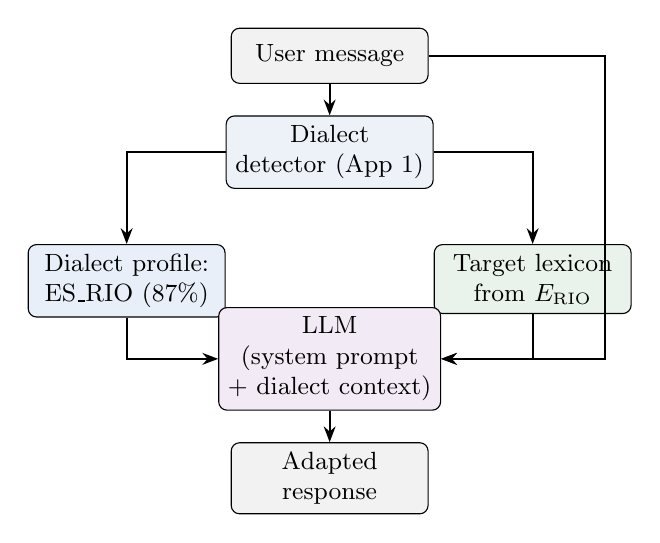
\begin{tikzpicture}[
  comp/.style={draw, rounded corners=3pt, minimum height=0.7cm,
               minimum width=2.5cm, font=\small, align=center},
  arr/.style={-{Stealth[length=2mm]}, thick},
  node distance=0.4cm and 0.8cm
]
\node[comp, fill=gray!10] (user) {User message};
\node[comp, fill=dialectA!10, below=of user] (detect) {Dialect\\detector (App 1)};
\node[comp, fill=appblue!10, below left=0.7cm and 0cm of detect] (profile) {Dialect profile:\\ES\_RIO (87\%)};
\node[comp, fill=appgreen!10, below right=0.7cm and 0cm of detect] (lexicon) {Target lexicon\\from $E_{\text{RIO}}$};
\node[comp, fill=apppurple!10, below=1.5cm of detect] (llm) {LLM\\(system prompt\\+ dialect context)};
\node[comp, fill=gray!10, below=of llm] (response) {Adapted\\response};

\draw[arr] (user) -- (detect);
\draw[arr] (detect) -| (profile);
\draw[arr] (detect) -| (lexicon);
\draw[arr] (profile) |- (llm);
\draw[arr] (lexicon) |- (llm);
\draw[arr] (user) -- ++(3.5,0) |- (llm);
\draw[arr] (llm) -- (response);
\end{tikzpicture}
\end{center}
\end{archbox}

\begin{howbox}{Adaptive generation}
\begin{enumerate}[nosep]
  \item \textbf{Detect dialect.} After 1--3 user messages, the
    dialect classifier has enough signal to identify the variety.

  \item \textbf{Build a dialect brief.} Using the word embeddings
    and eigenmode analysis, extract:
    \begin{itemize}[nosep]
      \item The top 100 most dialect-distinctive words for the
        detected variety.
      \item The pronoun and address system (voseo, tuteo, ustedeo).
      \item High-salience lexical pairs (``colectivo'' not ``bus'').
    \end{itemize}

  \item \textbf{Inject into LLM system prompt.} Pass the dialect
    brief to the LLM as a system instruction:
    \begin{quote}\small\itshape
    ``The user speaks Rioplatense Spanish. Use voseo (vos + ten\'es).
    Prefer: colectivo (not autob\'us), pileta (not piscina), frutilla
    (not fresa). Avoid Peninsular markers: vale, tío, mola.''
    \end{quote}

  \item \textbf{Post-filter.} After generation, scan the LLM output
    through the dialect scorer. If any words have high affinity for a
    \emph{different} dialect, replace them using the transfer mechanism
    (Application~3).
\end{enumerate}
\end{howbox}

% ----------------------------------------------------------------------
\section{Application 12: Synthetic Training Data Generation}
\label{sec:app-synthetic}
% ----------------------------------------------------------------------

\begin{appbox}[What it does]
Generate large volumes of dialect-labeled synthetic training data for
downstream NLP tasks (sentiment analysis, NER, intent classification)
where per-dialect annotated data is scarce.
\end{appbox}

\begin{howbox}{Dialect-controlled data augmentation}
\begin{enumerate}[nosep]
  \item \textbf{Start with labeled data in one dialect} (typically
    Peninsular or Mexican, where annotation resources are richest).

  \item \textbf{Transfer to target dialects} using Application~3's
    eigenmode-based lexical substitution.

  \item \textbf{Validate quality.} Run the generated texts through
    the dialect classifier (Application~1). Only keep texts that are
    classified as the target dialect with confidence $> 0.7$.

  \item \textbf{Train downstream models.} Use the synthetic data to
    fine-tune task-specific models (sentiment, NER, etc.) that
    generalize across dialects.
\end{enumerate}
\end{howbox}

This addresses a fundamental bottleneck in Spanish NLP: annotated
datasets exist primarily for Peninsular and Mexican Spanish. Training
on dialect-transferred synthetic data produces models that work for
Rioplatense, Caribbean, Andean, and other underresourced varieties.

% ----------------------------------------------------------------------
\section{Application 13: Forensic Author Profiling}
\label{sec:app-forensic}
% ----------------------------------------------------------------------

\begin{appbox}[What it does]
Given an anonymous text, estimate the author's geographic/dialectal
origin based on linguistic fingerprints encoded in the eigenmodes.
Goes beyond simple dialect classification by measuring the
\emph{strength and pattern} of dialectal features, not just the
most likely category.
\end{appbox}

\begin{howbox}{Spectral profiling}
\begin{enumerate}[nosep]
  \item \textbf{Embed and project.} Process the anonymous text
    through the model to get a 384-d centroid.

  \item \textbf{Full eigenmode activation.} For every variety's
    eigendecomposition, compute the full activation vector:
    $\mathbf{a}_v = P_v^{-1} \mathbf{c}$. This produces an 8-way
    set of 384-d activation profiles.

  \item \textbf{Activation fingerprint.} The pattern of which modes
    are activated and how strongly is a richer signal than a single
    classification. Two Rioplatense speakers may both be classified
    as ES\_RIO, but their mode activation patterns differ---one may
    show strong lunfardo (slang) modes, another strong academic register.

  \item \textbf{Confidence calibration.} The eigenvalue magnitudes
    provide natural uncertainty: modes with large eigenvalues
    contribute reliable signal; modes with small eigenvalues are noise.
    The system reports per-mode confidence alongside the profile.

  \item \textbf{Mixture detection.} If the activation profile is
    strongly bimodal (high activations for two different dialects'
    modes), the text may be from a bidialectal speaker or a
    code-switcher. The spectral profile naturally captures this.
\end{enumerate}
\end{howbox}

% ======================================================================
\part{Interactive and Educational Applications}
% ======================================================================

% ----------------------------------------------------------------------
\section{Application 14: Interactive Dialect Explorer}
\label{sec:app-explorer}
% ----------------------------------------------------------------------

\begin{appbox}[What it does]
A web application where users type or paste Spanish text and see a
real-time visualization of where it falls in dialect space: a 2D
projection of the 384-d space with the eight dialect clusters visible,
the input text's position highlighted, and the most diagnostic words
annotated.
\end{appbox}

\begin{howbox}{Interactive visualization}
\begin{enumerate}[nosep]
  \item \textbf{Pre-compute a 2D map.} Use t-SNE or UMAP on a
    sample of per-dialect sentence embeddings to create a 2D
    projection. The eight dialect clusters form visible regions.

  \item \textbf{Embed user input.} When the user types, process
    through the model and project to 2D using the pre-fitted
    projection.

  \item \textbf{Animate.} Show the input text's dot moving in
    real-time as the user types. As they add dialectally marked
    words, the dot shifts toward the corresponding cluster.

  \item \textbf{Annotate.} Highlight the words in the input that
    are most responsible for the current position (highest per-word
    dialect affinity). Color-code them by which dialect they pull
    toward.

  \item \textbf{Eigenmode drill-down.} Clicking a dialect cluster
    reveals its top eigenmodes and their characteristic vocabulary.
\end{enumerate}
\end{howbox}

% ----------------------------------------------------------------------
\section{Application 15: Dialectology Teaching Platform}
\label{sec:app-teaching}
% ----------------------------------------------------------------------

\begin{appbox}[What it does]
An educational tool that teaches students about Spanish dialectal
variation through interactive exercises powered by the v3 artifacts.
\end{appbox}

\subsection{Exercise types}

\begin{enumerate}
  \item \textbf{``Guess the dialect.''} Present a sentence; the
    student guesses the dialect. The system reveals the answer and
    highlights the diagnostic features, linking each to the eigenmode
    that captures it.

  \item \textbf{``Translate the dialect.''} Present a sentence in one
    variety; the student rewrites it in another. The system uses
    Application~3 to evaluate the rewrite, scoring each substitution
    against the eigenmode-predicted target word.

  \item \textbf{``Dialect continuum.''} The student places 8 dialect
    samples on a 2D map based on perceived similarity. The system
    compares their layout to the eigenv3 spectral distance matrix,
    revealing which similarities they perceived correctly and which
    they missed.

  \item \textbf{``Feature explorer.''} The student selects a
    linguistic feature (e.g., seseo, voseo, aspiration of
    /s/) and sees which eigenmodes capture it, which dialects
    exhibit it, and example sentences from the corpus.

  \item \textbf{``Build a dialect.''} Using the dialect algebra
    (Application~8), the student adjusts sliders for each eigenmode
    to construct a synthetic dialect, then sees what vocabulary
    characterizes their creation. This builds intuition for how
    dialectal features combine.
\end{enumerate}

% ======================================================================
\newpage
\part{Implementation Roadmap}
% ======================================================================

% ----------------------------------------------------------------------
\section{Artifact Dependencies and Build Order}
\label{sec:roadmap}
% ----------------------------------------------------------------------

\begin{center}
\renewcommand{\arraystretch}{1.3}
\begin{tabular}{>{\small}c >{\small}l >{\small}p{3.5cm} >{\small}p{5cm}}
\toprule
\textbf{Tier} & \textbf{Application} & \textbf{Required artifacts}
& \textbf{New code needed} \\
\midrule
\multirow{3}{*}{1}
  & Dialect identification & Model, scorer &
    FastAPI wrapper, batch endpoint \\
  & Dialect-aware filtering & + moderation lexicons &
    Per-dialect valence annotations \\
  & Recommendation & Classifier only &
    User profile accumulator \\
\midrule
\multirow{3}{*}{2}
  & Cross-dialectal search & $W_v$, $E_v$ &
    Reference-space indexer, vector DB \\
  & Content localization & $W_v$, $E_v$, eigenmodes &
    Review UI, translation memory \\
  & Chatbot adaptation & Classifier + eigenmodes &
    LLM system prompt generator \\
\midrule
\multirow{3}{*}{3}
  & Dialect transfer & $W_v$, $E_v$, morphology rules &
    Rule engine, post-editor \\
  & Synthetic data gen. & Transfer + classifier &
    Quality filter, task adapters \\
  & Author profiling & Full eigendecomposition &
    Activation fingerprint DB \\
\midrule
\multirow{4}{*}{4}
  & Dialectometry & Spectra, eigenmodes &
    Visualization pipeline \\
  & Dialect algebra & Algebra module &
    Interactive UI \\
  & Diachronic simulation & Multi-period spectra &
    Temporal corpus pipeline \\
  & Teaching platform & All of the above &
    Exercise engine, gamification \\
  & Interactive explorer & Model + 2D projection &
    Frontend (D3.js / Three.js) \\
\bottomrule
\end{tabular}
\end{center}

\subsection{Tier 1: Immediate (days)}

Applications 1, 2, and 6 require only the trained model and the
existing \texttt{DialectScorer} class. The code already exists in
\texttt{src/eigen3/scorer.py}; wrapping it in a REST API is
straightforward. This is the fastest path to a usable product.

\subsection{Tier 2: Short-term (weeks)}

Applications 5, 4, and 11 add the transformation matrices and
eigenmodes. The analysis pipeline (\texttt{transformation.py},
\texttt{decomposition.py}, \texttt{analyzer.py}) already computes
these. The new work is integration: building the reference-space
index for search, the review UI for localization, and the LLM prompt
generator for the chatbot.

\subsection{Tier 3: Medium-term (weeks to months)}

Applications 3, 12, and 13 require the dialect transfer pipeline,
which combines eigenmode-based lexical substitution with
morphological rules. The eigenmode part exists; the morphological
rule engine is new.

\subsection{Tier 4: Long-term (months)}

Applications 7--10 and 14--15 are research and educational tools
that require the full artifact stack plus visualization frontends.
The analytical backend (\texttt{analyzer.py}, \texttt{algebra.py})
already implements most of the mathematics; the work is in building
interactive interfaces.

% ======================================================================
\newpage
\part*{Summary: The Application Landscape}
\addcontentsline{toc}{part}{Summary}
% ======================================================================

\begin{center}
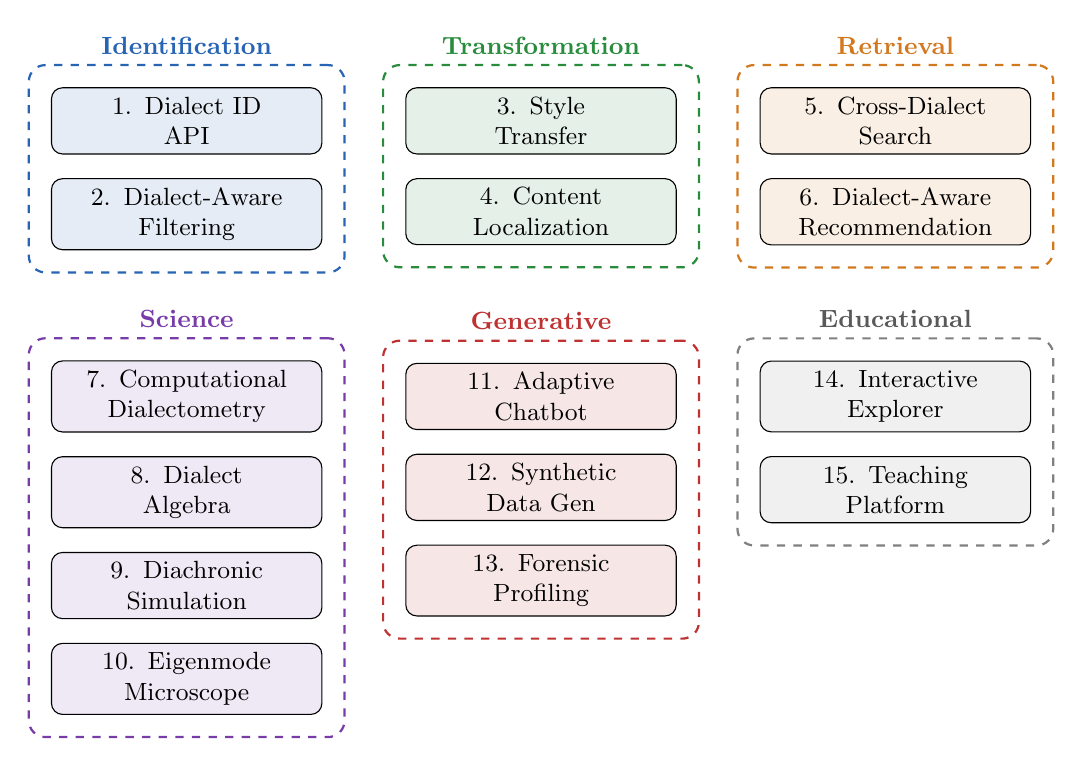
\begin{tikzpicture}[
  app/.style={draw, rounded corners=4pt, minimum height=0.6cm,
              font=\small, align=center, text width=3.2cm},
  domainbox/.style={draw, rounded corners=6pt, thick, dashed,
                 inner sep=8pt},
  node distance=0.3cm
]

% Identification
\node[app, fill=appblue!12] (a1) at (0,0) {1. Dialect ID\\API};
\node[app, fill=appblue!12, below=of a1] (a2) {2. Dialect-Aware\\Filtering};
\node[domainbox, appblue, fit=(a1)(a2),
      label={[font=\small\bfseries, appblue]above:Identification}] {};

% Transformation
\node[app, fill=appgreen!12] (a3) at (4.5,0) {3. Style\\Transfer};
\node[app, fill=appgreen!12, below=of a3] (a4) {4. Content\\Localization};
\node[domainbox, appgreen, fit=(a3)(a4),
      label={[font=\small\bfseries, appgreen]above:Transformation}] {};

% Retrieval
\node[app, fill=apporange!12] (a5) at (9,0) {5. Cross-Dialect\\Search};
\node[app, fill=apporange!12, below=of a5] (a6) {6. Dialect-Aware\\Recommendation};
\node[domainbox, apporange, fit=(a5)(a6),
      label={[font=\small\bfseries, apporange]above:Retrieval}] {};

% Science
\node[app, fill=apppurple!12] (a7) at (0,-3.5) {7. Computational\\Dialectometry};
\node[app, fill=apppurple!12, below=of a7] (a8) {8. Dialect\\Algebra};
\node[app, fill=apppurple!12, below=of a8] (a9) {9. Diachronic\\Simulation};
\node[app, fill=apppurple!12, below=of a9] (a10) {10. Eigenmode\\Microscope};
\node[domainbox, apppurple, fit=(a7)(a8)(a9)(a10),
      label={[font=\small\bfseries, apppurple]above:Science}] {};

% Generative
\node[app, fill=appred!12] (a11) at (4.5,-3.5) {11. Adaptive\\Chatbot};
\node[app, fill=appred!12, below=of a11] (a12) {12. Synthetic\\Data Gen};
\node[app, fill=appred!12, below=of a12] (a13) {13. Forensic\\Profiling};
\node[domainbox, appred, fit=(a11)(a12)(a13),
      label={[font=\small\bfseries, appred]above:Generative}] {};

% Educational
\node[app, fill=gray!12] (a14) at (9,-3.5) {14. Interactive\\Explorer};
\node[app, fill=gray!12, below=of a14] (a15) {15. Teaching\\Platform};
\node[domainbox, gray, fit=(a14)(a15),
      label={[font=\small\bfseries, gray!70!black]above:Educational}] {};

\end{tikzpicture}
\end{center}

\bigskip

EigenDialectos v3 is not merely a classifier or an embedding model.
Its spectral decomposition of dialect space creates a mathematical
framework in which dialects become objects that can be
\textbf{measured} (distances, effective rank),
\textbf{compared} (shared vs.\ unique eigenmodes),
\textbf{transformed} (one dialect to another via $W^{-1}_s W_t$),
\textbf{composed} (weighted spectral sums),
\textbf{interpolated} (continuous paths between dialects), and
\textbf{inverted} (anti-dialects, impossible varieties).

Each of the 15 applications described in this document exploits one or
more of these operations. The artifacts are already computed; the
applications are architecture and integration.

\end{document}
